%-------------------------------------------------------------------------------
%                                PREAMBLE
%-------------------------------------------------------------------------------
\documentclass[usenames,dvipsnames,svgnames,10pt,aspectratio=169]{beamer}
\usefonttheme{professionalfonts}

% This theme uses TIKZ: compile twice with PDFLaTeX or LuaLaTeX.
%
%  Options:
%  - [clean]:    clean slides, i.e. logos and footbar are removed
%  - [kth]:      footbar style inspierd to the official KTH template
%  - [nicewave]: a different style of wave is used (not approved by FLOW)
%
\usetheme{flow}

\usepackage{hyperref,graphicx,lmodern}
\usepackage[utf8]{inputenc}
\usepackage{media9}
\usepackage{xcolor}
\usepackage{stmaryrd}
\usepackage{nicefrac}
\usepackage{multimedia}
\usepackage{multicol}
\usepackage{upgreek}
\usepackage[]{bm}
\usepackage[]{url}

\DeclareMathOperator{\sinc}{sinc}
\DeclareMathAlphabet{\mathcal}{OMS}{cmsy}{m}{n}
\DeclareMathAlphabet\mathbfcal{OMS}{cmsy}{b}{n}

\graphicspath{{imgs/}}
\setbeamertemplate{blocks}[rounded][shadow=true]

\DeclareMathOperator{\trace}{tr}

%-------------------------------------------------------------------------------
%                                TITLE PAGE
%-------------------------------------------------------------------------------
\title[Nonlinear Physics] % Short title used in footline
{
	Nonlinear physics, dynamical \\ systems and chaos theory
}

\author[J.-Ch.~Loiseau] % Presenting author in short form used in footline
{
	Jean-Christophe Loiseau
}
% - Give the names in the same order as the appear in the paper.
% - Underline the presenting author.

\institute[unused]
{
	\url{jean-christophe.loiseau@ensam.eu} \\
	DynFluid, \\
	Arts et M\'etiers ParisTech, France
}
% Keep it simple, no one is interested in your street address.

% University logo(s)
\logot{
\includegraphics[width=.128\paperwidth]{DynFluid_logo}}  % Top logo
\logob{
\includegraphics[width=0.128\paperwidth]{ENSAM_logo}} % Bottom logo
% \logoc[{
\includegraphics[width=.128\paperwidth]{limsi}}]{
\includegraphics[width=.128\paperwidth]{limsi}} % Corner logo
%
% Cover image: \cvrimg{x position}{y position}{cover image}
\cvrimg{.77}{.8}{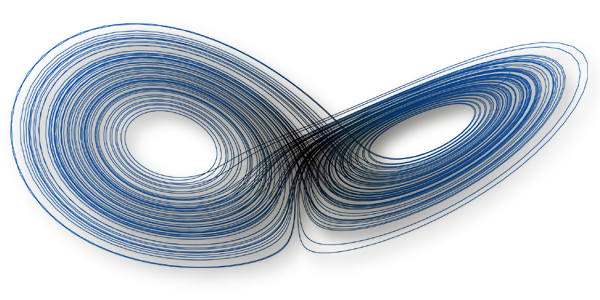
\includegraphics[width=.4\paperwidth]{cover.png}}

\date[unused]{ENSAM, Master 2, 2017--2018}

\begin{document}

\titleframe % Print the title as the first slide

%-------------------------------------------------------------------------------
%                           PRESENTATION SLIDES
%-------------------------------------------------------------------------------

\begin{frame}[t, c]{}{}

\end{frame}

\begin{frame}[t, c]{Today's menu}{The different routes to chaos}
	\begin{itemize}
		\item So far, we have seen at least two sequences of bifurcations that cause a system to exhibit chaotic dynamics.
		\begin{itemize}
			\item[$\hookrightarrow$] \alert{\textbf{Logistic map}}: Sequence of period doubling bifurcations.
			\item[$\hookrightarrow$] \alert{\textbf{Lorenz system}}: For $0 \leq \rho \leq 25$, a supercritical pitchfork and a subcritical Hopf bifurcations occur before the creation of a stange attractor.
		\end{itemize}

		\bigskip

		\item These are two different routes to chaos. They are not the only ones though...
	\end{itemize}

	\vspace{1cm}
\end{frame}

\begin{frame}[t, c]{}
	\centering
	\vspace{1cm}

	{\Large \textbf{The routes to chaos}}

	\bigskip

	{\textgre{\textbf{Subharmonic cascade}}}

\end{frame}

\begin{frame}[t, c]{Subharmonic cascade}{Logistic map}
	\begin{itemize}
		\item Let us consider once again the logistic map given by
		$$x_{k+1} = \mu x_k ( 1 - x_k),$$
		where $\mu$ is our control parameters.

		\bigskip

		\item We have studied this discrete-time system during Lecture 5.
	\end{itemize}

	\vspace{1cm}
\end{frame}

\begin{frame}[t, c]{Logistic map}{Cobweb and phase plane for $\mu = 1$}
	\begin{minipage}{.48\textwidth}
		\centering
		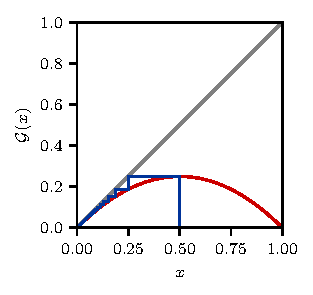
\includegraphics[width=.75\textwidth]{logistic_map_cobweb_plot_0}
	\end{minipage}%
	\begin{minipage}{.48\textwidth}
		\centering
		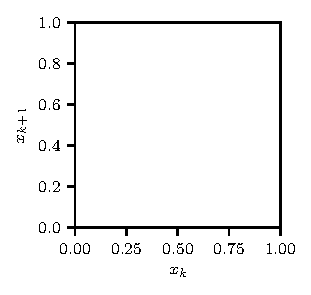
\includegraphics[width=.75\textwidth]{logistic_map_phase_plane_0}
	\end{minipage}

	\vspace{1cm}
\end{frame}

\begin{frame}[t, c]{Logistic map}{Cobweb and phase plane for $\mu = 1.32$}
	\begin{minipage}{.48\textwidth}
		\centering
		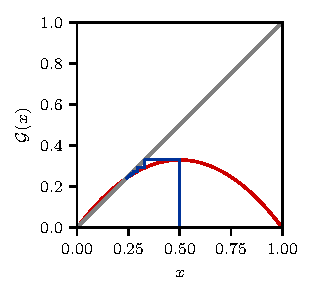
\includegraphics[width=.75\textwidth]{logistic_map_cobweb_plot_1}
	\end{minipage}%
	\begin{minipage}{.48\textwidth}
		\centering
		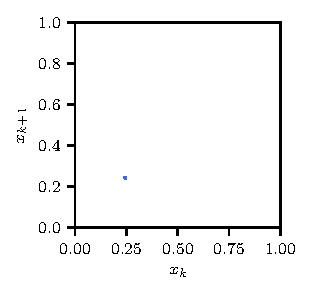
\includegraphics[width=.75\textwidth]{logistic_map_phase_plane_1}
	\end{minipage}

	\vspace{1cm}
\end{frame}

\begin{frame}[t, c]{Logistic map}{Cobweb and phase plane for $\mu = 1.64$}
	\begin{minipage}{.48\textwidth}
		\centering
		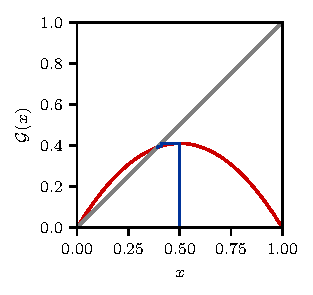
\includegraphics[width=.75\textwidth]{logistic_map_cobweb_plot_2}
	\end{minipage}%
	\begin{minipage}{.48\textwidth}
		\centering
		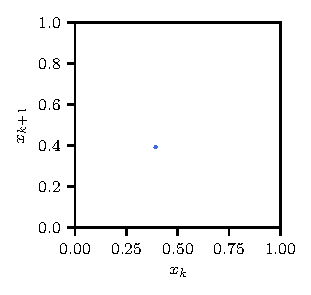
\includegraphics[width=.75\textwidth]{logistic_map_phase_plane_2}
	\end{minipage}

	\vspace{1cm}
\end{frame}

\begin{frame}[t, c]{Logistic map}{Cobweb and phase plane for $\mu = 1.96$}
	\begin{minipage}{.48\textwidth}
		\centering
		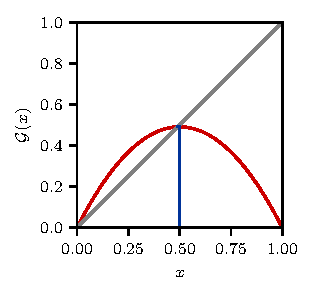
\includegraphics[width=.75\textwidth]{logistic_map_cobweb_plot_3}
	\end{minipage}%
	\begin{minipage}{.48\textwidth}
		\centering
		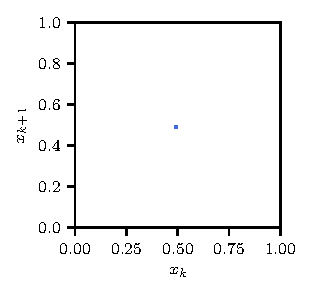
\includegraphics[width=.75\textwidth]{logistic_map_phase_plane_3}
	\end{minipage}

	\vspace{1cm}
\end{frame}

\begin{frame}[t, c]{Logistic map}{Cobweb and phase plane for $\mu = 2.28$}
	\begin{minipage}{.48\textwidth}
		\centering
		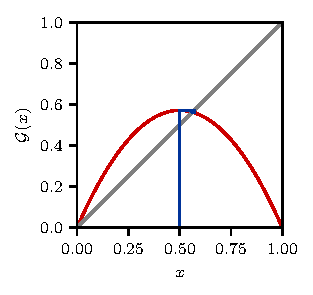
\includegraphics[width=.75\textwidth]{logistic_map_cobweb_plot_4}
	\end{minipage}%
	\begin{minipage}{.48\textwidth}
		\centering
		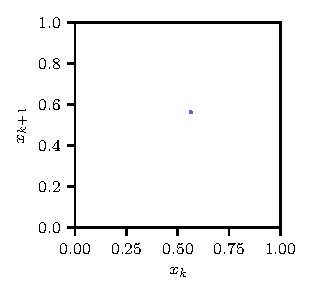
\includegraphics[width=.75\textwidth]{logistic_map_phase_plane_4}
	\end{minipage}

	\vspace{1cm}
\end{frame}

\begin{frame}[t, c]{Logistic map}{Cobweb and phase plane for $\mu = 2.61$}
	\begin{minipage}{.48\textwidth}
		\centering
		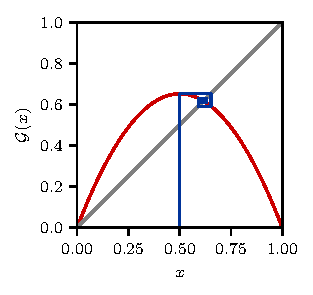
\includegraphics[width=.75\textwidth]{logistic_map_cobweb_plot_5}
	\end{minipage}%
	\begin{minipage}{.48\textwidth}
		\centering
		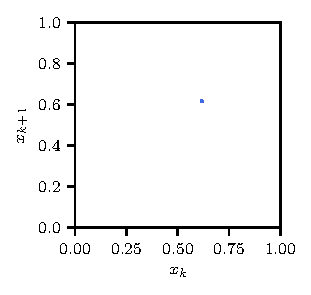
\includegraphics[width=.75\textwidth]{logistic_map_phase_plane_5}
	\end{minipage}

	\vspace{1cm}
\end{frame}

\begin{frame}[t, c]{Logistic map}{Cobweb and phase plane for $\mu = 2.93$}
	\begin{minipage}{.48\textwidth}
		\centering
		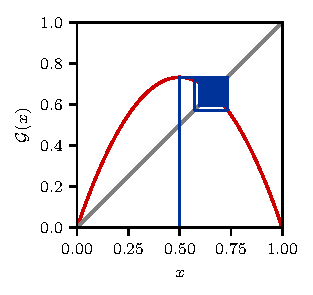
\includegraphics[width=.75\textwidth]{logistic_map_cobweb_plot_6}
	\end{minipage}%
	\begin{minipage}{.48\textwidth}
		\centering
		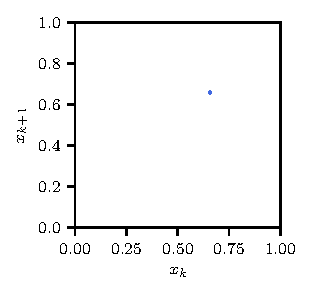
\includegraphics[width=.75\textwidth]{logistic_map_phase_plane_6}
	\end{minipage}

	\vspace{1cm}
\end{frame}

\begin{frame}[t, c]{Logistic map}{Cobweb and phase plane for $\mu = 3.25$}
	\begin{minipage}{.48\textwidth}
		\centering
		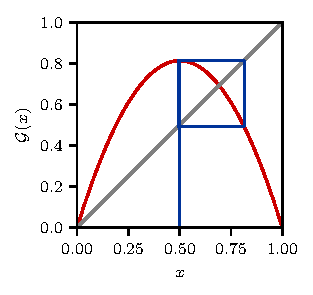
\includegraphics[width=.75\textwidth]{logistic_map_cobweb_plot_7}
	\end{minipage}%
	\begin{minipage}{.48\textwidth}
		\centering
		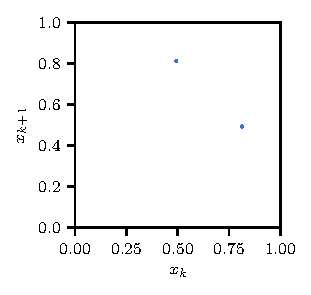
\includegraphics[width=.75\textwidth]{logistic_map_phase_plane_7}
	\end{minipage}

	\vspace{1cm}
\end{frame}

\begin{frame}[t, c]{Logistic map}{Cobweb and phase plane for $\mu = 3.57$}
	\begin{minipage}{.48\textwidth}
		\centering
		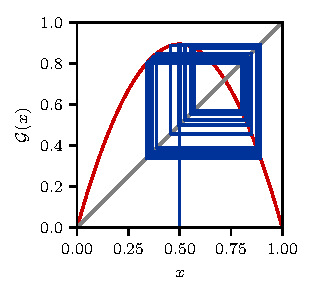
\includegraphics[width=.75\textwidth]{logistic_map_cobweb_plot_8}
	\end{minipage}%
	\begin{minipage}{.48\textwidth}
		\centering
		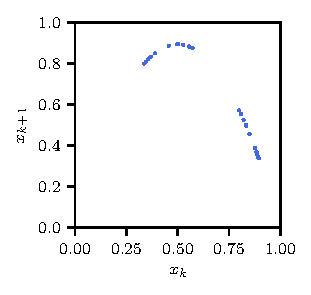
\includegraphics[width=.75\textwidth]{logistic_map_phase_plane_8}
	\end{minipage}

	\vspace{1cm}
\end{frame}

\begin{frame}[t, c]{Logistic map}{Cobweb and phase plane for $\mu = 3.9$}
	\begin{minipage}{.48\textwidth}
		\centering
		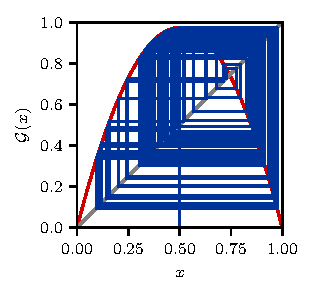
\includegraphics[width=.75\textwidth]{logistic_map_cobweb_plot_9}
	\end{minipage}%
	\begin{minipage}{.48\textwidth}
		\centering
		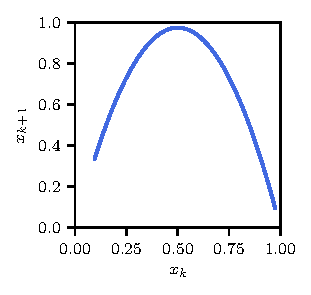
\includegraphics[width=.75\textwidth]{logistic_map_phase_plane_9}
	\end{minipage}

	\vspace{1cm}
\end{frame}

\begin{frame}[t, c]{Logistic map}{Bifurcation diagram}
	\centering
	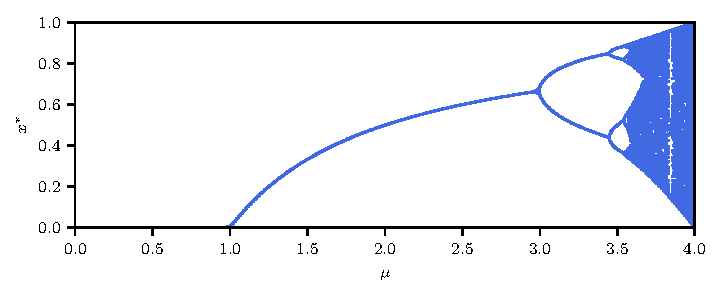
\includegraphics[width=.75\textwidth]{logistic_map_bifurcation_overview}

	\vspace{1cm}
\end{frame}

\begin{frame}[t, c]{Logistic map}{Bifurcation diagram}
	\centering
	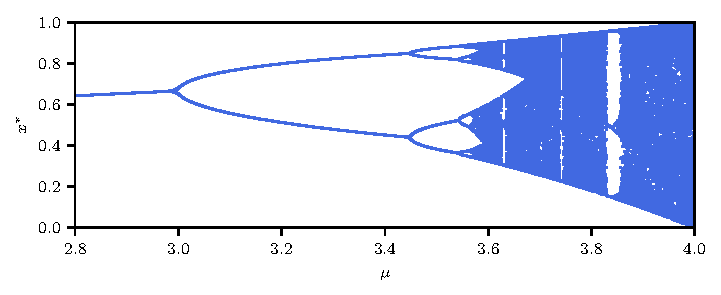
\includegraphics[width=.75\textwidth]{logistic_map_bifurcation_zoom_1}

	\vspace{1cm}
\end{frame}

\begin{frame}[t, c]{Logistic map}{Subharmonic cascade}
	\begin{itemize}
		\item Let us verify "experimentally" that the sequence of bifurcations taking place indeed corresponds to a subharmonic cascade.

		\bigskip

		\item For that purpose, we will analyze time-series of $x_{k}$ for different values of $\mu$ using the \emph{discrete Fourier transform}.
	\end{itemize}

	\vspace{1cm}
\end{frame}

\begin{frame}[t, c]{Logistic map}{Subharmonic cascade}

\end{frame}

\begin{frame}[t, c]{Logistic map}{Subharmonic cascade}
	\begin{itemize}
		\item At each bifurcation point, the period of the limit cycle doubles.
		\begin{itemize}
			\item[$\hookrightarrow$] $\mu_1 = ?? \to$ period 1.
			\item[$\hookrightarrow$] $\mu_2 = ?? \to$ period 2.
			\item[$\hookrightarrow$] $\mu_3 = ?? \to$ period 4.
			\item[$\hookrightarrow$] $\mu_4 = ?? \to$ period 8.
			\item[$\hookrightarrow$] ...
		\end{itemize}

		\bigskip

		\item This scenario is not limited to discrete-time dynamical systems, but can also occurs in continuous-time systems.
	\end{itemize}

	\vspace{1cm}
\end{frame}

\begin{frame}[t, c]{R\"ossler system}{A "simplified" Lorenz model}
	\begin{itemize}
		\item In 1976, Otto R\"ossler introduced this "simplified" version of Lorenz model
		\begin{equation}
			\begin{aligned}
				\dot{x} & = -y -z \\
				\dot{y} & = x + a y \\
				\dot{z} & = b + z(x-c).
			\end{aligned}
			\notag
		\end{equation}
		where we will assume $a=b=0.2$, while $c$ will be our control parameter.

		\bigskip

		\item Although its original goal was purely theoretical, this model has since then proven able to describe a certain class of chemical reactions.
	\end{itemize}

	\vspace{1cm}
\end{frame}

\begin{frame}[t, c]{R\"ossler system}{Subharmonic cascade}

\end{frame}

\begin{frame}[t, c]{R\"ossler system}{Bifurcation diagram}

\end{frame}

\begin{frame}[t, c]{R\"ossler system}{Subharmonic cascade}
		\begin{itemize}
			\item As before, the period of the limit cycle doubles at each bifurcation point.
			\begin{itemize}
				\item[$\hookrightarrow$] $c_1 = ?? \to$ period 1.
				\item[$\hookrightarrow$] $c_2 = ?? \to$ period 2.
				\item[$\hookrightarrow$] $c_3 = ?? \to$ period 4.
				\item[$\hookrightarrow$] $c_4 = ?? \to$ period 8.
				\item[$\hookrightarrow$] ...
			\end{itemize}

			\bigskip

			\item Deep down, the transition to chaos for the R\"ossler system obeys the same law as the transition to chaos for the logistic map.
		\end{itemize}

		\vspace{1cm}
\end{frame}

\begin{frame}[t, c]{Lorenz system}{Low-order model for thermal convection}
	\begin{itemize}
		\item Let us once more consider the Lorenz system
		\begin{equation}
			\begin{aligned}
				\dot{x} & = \sigma ( y - x )\\
				\dot{y} & = x(\rho -z) - y \\
				\dot{z} & = xy - \beta z,
			\end{aligned}
			\notag
		\end{equation}
		where we set $\sigma=10$ and $\beta = \nicefrac{8}{3}$.

		\bigskip

		\item The transition to chaos when $\rho$ varies from $0$ to $28$ has been studied in Lecture 6.

		\bigskip

		\item For the moment, we will now draw our attention when $\rho$ varies from 313 down to 215.
	\end{itemize}

	\vspace{1cm}
\end{frame}

\begin{frame}[t, c]{Lorenz system}{Bifurcation diagram}

\end{frame}

\begin{frame}[t, c]{Lorenz system}{Subharmonic cascade}

\end{frame}

\begin{frame}[t, c]{Lorenz system}{Subharmonic cascade}
		\begin{itemize}
			\item Once more, the period of the limit cycle doubles at each bifurcation point.
			\begin{itemize}
				\item[$\hookrightarrow$] $\rho_1 = ?? \to$ period 1.
				\item[$\hookrightarrow$] $\rho_2 = ?? \to$ period 2.
				\item[$\hookrightarrow$] $\rho_3 = ?? \to$ period 4.
				\item[$\hookrightarrow$] $\rho_4 = ?? \to$ period 8.
				\item[$\hookrightarrow$] ...
			\end{itemize}

			\bigskip

			\item Again, the transition to chaos for $215 \leq \rho \leq 313$ is very similar to that of the logistic map and of the R\"ossler system.
		\end{itemize}

		\vspace{1cm}
\end{frame}

\begin{frame}[t, c]{Subharmonic cascade}{}
	\begin{block}{\centering \textbf{Question}}
		\centering
		How similar are these different systems?
	\end{block}
\end{frame}

\begin{frame}[t, c]{Subharmonic cascade}{}

\end{frame}

\begin{frame}[t, c]{Subharmonic cascade}{}
		\begin{center}
			\begin{tabular}{cccccc}
				~ & $\nicefrac{\mu_3-\mu_2}{\mu_2 - \mu_1}$ &$\nicefrac{\mu_4-\mu_3}{\mu_3 - \mu_2}$ &$\nicefrac{\mu_5-\mu_4}{\mu_4 - \mu_3}$ &$\nicefrac{\mu_6-\mu_5}{\mu_5 - \mu_4}$ &$\nicefrac{\mu_7-\mu_6}{\mu_6 - \mu_5}$ \\
				Logistic map & $??$ & $??$ & $??$ & $??$ & $??$ \\
				R\"ossler & $??$ & $??$ & $??$ & $??$ & $??$ \\
				Lorenz & $5.019923$ & $4.710117$ & $4.671428$ & $4.669227$ & $4.669203$
			\end{tabular}
		\end{center}

		\vspace{1cm}
\end{frame}

\begin{frame}[t, c]{Subharmonic cascade}{}
	\begin{itemize}
		\item In all cases, the sequence
		$$\delta_i = \displaystyle \frac{\mu_{i} - \mu_{i-1}}{\mu_{i-1} - \mu_{i-2}}$$
		converges to $??$.

		\bigskip

		\item This number is known as ?? and is the signature of the subharmonic cascade.
	\end{itemize}

	\vspace{1cm}
\end{frame}

\begin{frame}[t, c]{}
	\centering
	\vspace{1cm}

	{\Large \textbf{The routes to chaos}}

	\bigskip

	{\textgre{\textbf{??}}}

\end{frame}

\end{document}
